\chapter{科学的推論}
科学におけるモデルおよび、数理統計学におけるモデルについて説明し、その違いを明らかにする。


\section{モデル}
モデル(模型)とは、現実を表していると思わせるような、作られたものであり、次の特徴を備えています。
\begin{enumerate}
    \item モデルは本物の特徴の一部を推測可能。本物との乖離の程度も推測できる
    \item (1)を行うために、複数の仮定により構築される。また、それらの仮定は、現状の知識では明らかではないまたは、現実的には成立していないことがある。
    %推測可能なことを増やすために仮定を増やすことがある。
    % \item モデルは本物の要素・特徴の全体を推測することはできない。
    \item モデルは間違った推測をする。
\end{enumerate}
  
例えば、車のプラモデルはモデルの一つです。本物の特徴の一つである大きさを推測可能にするため、スケール(例えば、1/24など)を決めて作られている。ドアや車体の幅を計測し、スケール倍すれば、本物の大きさを推測できる。普段長さを測れない場所であっても、手のひらに収まるプラモデルであれば、どの部分でも推測が可能になる。言い換えれば、本物の車がなくても、スケールを維持した車のプラモデルを持っていれば、簡単に大きさに関する推測が可能になる。



\if 0
モデルの仮定によって推測可能なことが増えることがある。
例えば、本物のパーツの重量に応じて、モデルのパーツの重さを変化させる。
こうすることで、プラスティックでできたモデルの重さを計測すると、そこから本物の重さの推測が可能になる。
他にも推測したいこと、例えば、素材の質感や色や重量、または車の速度といった特徴なども、モデルに仮定を追加することで、本物の様子を捉えることが可能になっていく。
\fi

本物の車を持って来れば、本物の様子を推測することが可能であるので、本物の車は、車自身のモデルということができるが、車を車自身のモデルとすると、それまであった利便性が損なわれる。
%また、モデルの仮定を増やせば、本物の車にモデルを近づけることが可能である。
おおよその車体の長さが知りたいのに、わざわざ長い測りが必要になることや、手に持って観察することもできない。
このように、細部まで推測可能にするというのは、デメリットになることがあり、モデルとして利用することはない。

細部まで推測可能なモデルは使うことは稀であり、車のモデルとして、大きさの尺度を保っていない直方体のブロックを使うことがある。このモデルでも推測できることがある。3台の同じ車を縦列駐車するのに必要な長さなどは、直方体三つ分と推測が可能である。
モデルの作り込みの程度によって車の特徴に関して推測できることの種類が決まる。
%が異なる。統計学を利用するときは、目的について考えることは少なく、儀式的に採用した手順に従うことが多い。

真球を車のモデルし、車の大きさに関する推測を行うと、現実の大きさと推測は大きく乖離することが考えられる。
モデルが本物の推測に使えないということに判断を下すには、本物のデータとモデルの出す推測を複数の指標から比較し考察することになる。


軽自動車に対してその大きさを予測可能なモデルを使って、トラックの大きさを予測できる。
予測できるが、その予測値は実際のトラックの大きさと異なる。
モデルが車体長を3.4mであると予測される。実際のトラックの車体長は6mよりも大きい。
メートル単位でモデルと実際には差が生じる。
このように、モデルと実際を調べることで、このモデルではトラックの大きさを推測できないと判定できる。
実際には、どれくらいの誤差が生じたときに、モデルが使えないというのかは、予測したいことにより異なる。

%車のモデルという題材からモデルの特徴を挙げた

モデルは本物ではないが、推測に役にたつ物として利用する。モデルと本物が極めて一致するように感じられることもあると思うが、モデルは本物ではない。



\section{統計モデル}
統計モデルについて説明し、モデルを使って現実を推測することを概念図を用いて説明する。
まず、統計モデルは、数理統計の知識を使いモデルを構築され、現実を推測するために用いられる。簡単な統計モデルを例に挙げると、次のような仮説から構築される。

\begin{enumerate}
    \item (仮定1)確率変数が同一の分布から独立に得られる(i.i.d)
    \item (仮定2)その分布関数は、$f(x)$と書ける。
    \item (仮定3)分布関数の母数に関する仮説\footnote{三番目の仮説のみを統計モデルと主張する流派もある\cite{塩見_正衛2021}}
\end{enumerate}

\subsection{統計モデルとデータ}
%統計モデルは予測を
データに統計モデルがよく当てはまるよう指標を定め、その指標を小さくするようにモデルの母数を推定できる。



\subsection{データへの過剰適合}
モデルは改訂することにより、予測の精度をあげることができた。これは、何度も対象を観測することで、モデルと実際の当てはまりを定量的な評価が可能であるから、モデルの作り込みを防ぐことができる。
再現性の確保されている現象に対しては、データに当てはまるようにモデルに仮定を足していき、モデルの作り込みを行う。さらに新たなデータとモデルの予測とを定量的な指標を元に評価する。
一方で、何度も繰り返し観測可能でない現象を対象にした学問領域において、モデルの作り込みは現在得られているデータを過度によく予測するモデルとなることがある。その結果、構築したモデルが新に得たデータに対して予測精度が落ちてしまうことが多々ある。
そのため、データを見た後に、モデルに仮定の追加または変更はしない方が良い。




\subsection{統計モデルの仮定を自然が満たしているのか}
統計モデルにより推定したい対象またはデータが、統計モデルの仮定から外れていることは多々ある。
まず仮定1、独立性と同一の分布という仮定は、数学的厳密な定義がある。
その定義を現実の世界にの言葉に変換すること自体が難しい。
まず、各変数が独立とは、事象A,Bが同時に起きた確立$P(A,B)$がそれぞれが生じる確率の積に等しいということであり、$P(A,B)=P(A)P(B)$である。そもそも事象生じる頻度が$P$により決定されているということを考えることができない。それに加えて$P(A,B)=P(A)P(B)$なども、現実世界の事象に一致する概念がない。
%\footnote{同様のものとして、尤度も現実に対応する概念がない。よく尤もらしさと言い換えられるが、間違っている。尤度は$P(A)P(B)P(C)\cdots$である。それ以外の言い換えは間違いである。}。

間違っていることを承知の上で、科学的な言葉に変換して、妥当であるかを考察してみる。
あえて、得られたデータに相関が全くないと、捉えてみると、現実的には妥当ではないことの方が多い。例えば、人の身長を計測器により繰り返し観測すると、その計測器や扱う人の癖がデータに含まれ、それはデータの傾向を決定する因子となり、データ間には相関があると考えられる。
もし、相関がない実験デザインを設定できたとしても、人の身長はその背景にある社会や遺伝的な繋がりが因子となっており、相関が無いと言い切ることは難しい。

同一の分布とは、同一の数学的規則に自然が支配されていることを仮定していると考えられる。コインのトスでは、その裏表の出現確率を二項分布によるものと考えても問題が大きくならない。一方で、人の身長は、母父の大きさや成長過程における栄養の量などの因子によって成長すると考えられる。この現象が、サイコロのように乱数をふって決定されていると考えるのは妥当とは言い切れない\footnote{そう考えてもいいけど、あまり役に立たない}。
%統計モデルの数学的な仮定が科学と対応しているとは言い難い。
%モデルは、妥当とは言い切れない仮定により構築されている。


統計モデルを現実の推測に使えないということではない。モデルと現象を比べて予測するためだけにモデルを利用するのであるから、仮定が現実に存在するかはどうでも良い。
\begin{SMbox}
    Boxらは、統計学において正規分布や一次関数で推論することを次のように捉えている\cite{box1976science}。
\begin{quote}
    Equally, the statistician knows, for example, that in nature there never was a normal distribution, there never was a straight line, yet with normal and linear assumptions, known to be false, he can often derive results which match, to a useful approximation, those found in the real world. 
\end{quote}
    %データが正規分布的に分布しているということは、ある中心に対して対照的にデータが生じていることを示す。このとき、正規分布でデータを予測するのが良いのではないかと考える。
\end{SMbox}
%以下では、統計モデルを$M(\bm{a})$とし、ここで$\bm{a}$は、仮定3の統計モデルの母数であり、母数が複数あることも考慮し、ベクトルで表記しておく。

\begin{SMbox}{学問間に生じているモデルに関する認識の違い}
モデルが本物であるか否かは、学問領域によって認識が異なっている。
私は、モデルは現実を推測するための偽物のことだと考えている。
モデルが自分の知りたいことをうまく予測してくれさえいればいいという立場である。
一方で、数学では、モデルを現実と捉える傾向がある。モデルにより世界が支配されていると考えているのである。例えば、ある数学者は、流体モデルに解が安定的に存在するかがわからないから飛行機に乗りたくないと思っていると言う雰囲気がある。
現代の統計学はどちらかと言うと数学者が作った枠組みを統計ユーザーが受け入れてしまったため、ユーザーたちは、数学者のように現象を捉ようとしているように見える。

実際にモデルに対する認識が研究者によって異なっていると感じている人はいる。
学習理論を研究しておられる渡邊 澄夫さんは、情報科学と物理学におけるモデルとして次のような見解を述べている。
\begin{quote}
    (注意)このことを聞いたとき,どのように感じるかは,人によって ずいぶん違います.情報科学の研究者の人たちは,「目的が違うのだから, 最適なものが違うのは当然であり,まったく不思議ではない」と感じる場合が多いようです. 一方,物理学の研究者の人たちは, 「真の法則が発見できるということと,最良の予測ができることとは,ぴったりと 同じであるべきである」と感じるようです.これは,おそらく,「モデル」という 概念や重みにおいて,情報科学と物理学では大きな隔たりがあることが原因ではないかと 思います.(例題:電子の質量が正確に予言できるのは,量子電磁力学が真の自然法則であるからと 考えられています).

    生物学・環境学・経済学に用いられる「モデル」は,上記の意味での情報科学におけるモデルに近いのか, 物理学における理論に近いのか,それとも,その中間に当たるのか,もっと違う種類の ものなのか,は,かなり微妙な質問で,一様な回答はないものと思います. 数学者のかたが数理科学の研究に挑もうとされるときには,「モデル」という言葉が表すものが, 分野において,場合において,このように様々に異なりうることを認識されておかれるとよろしいでしょう。
    \\ \url{http://watanabe-www.math.dis.titech.ac.jp/users/swatanab/Bayestheory2.html}
\end{quote}

統計や機械学習の分野で有名なBox氏は、「全てのモデルは間違いである(All models are wrong)」と、次のように説明している。
\if 0
\begin{quote}
    For such a model there is no need to ask the question "Is the model true?". If "truth" is to be the "whole truth" the answer must be "No". The only question of interest is "Is the model illuminating and useful?".
\end{quote}
\fi

\end{SMbox}


\if 0
\begin{mybox}
    %\begin{quotation}
    \paragraph{頻度主義・ベイズ主義}
    頻度主義・ベイズ主義は統計学の流派を表す言葉である。頻度主義者であると言う人はあまり見たことがないが、ベイズ主義者はよく見る。ベイズ主義者は頻度主義者を非難するような主張をすることが多々ある。それぞれの立場を正確に説明した文献がないので、何を意味しているのかを私は理解できていない。

    おそらく、頻度主義では、モデルと母集団を一致させて考えており、このことを念頭にすれば頻度主義的な議論が理解できると思う。この立場にたてば、中心極限定理がデータにも適応可能になり、あらゆるデータが正規分布で推定可能にることを主張できる\footnote{本当にそう考えているのか確信が持てない}。
    %\end{quotation}
\end{mybox}
\fi


\if 0
\begin{brokenbox}[colback=yellow]
    \blindtext[5]
  \end{brokenbox}
\fi 
\subsection{数理モデルの機能}
数理モデルには予測・サンプリングという機能がある。それぞれ説明していく。
\paragraph{予測}

次に説明するサンプリングを使うことで出現しやすい場所を数値的に計算することが必要となるモデルもある。

\paragraph{サンプリング}
サンプリングは、モデルを使ってデータを生成する方法である。モデルが説明したいデータの出現頻度をよく予測できるなら、モデルが生成したデータは実際に得られるデータと似たものになる。

\section{数理統計学におけるモデル}
数理統計学は、モデルが生成した有限個の確率変数からモデルの母数を推測する方法論を提供している。



\if 0
\subsubsection{オッカムの剃刀}

仮定の追加には合理的な理由が必要だと考えられます\footnote{仮定を追加した統計モデルはベイズ統計と書かれた本で学ことができます。}。

\begin{figure}
    \begin{center}
%\includesvg{../markdown/section1/statistics_model.svg}
\end{center}
\end{figure}
\fi
\section{統計学の用語}

\subsection{母集団、無作為抽出、サンプリング}
母集団は興味のある対象全体の集団のことである。例えば、17歳男性の身長に関心があるならば、17歳男性の全員の集合が母集団である。
無作為抽出とは、偏りなく母集団からデータを取得することである。
無作為抽出することで、都合の良い結果が集まらないようにしている\footnote{無作為抽出しなければならないのはモデルの仮定1を満たすためだという主張を見かけたことがある(文献を探すべき)。モデルの仮定を現実が満たすようにすることは難しいので、そのように考えなくて良い。}。
サンプリングは無作為抽出の英訳である。本書では、モデルからの無作為抽出のことをあえてサンプリングとカタカナで記述し、現実の作業である無作為抽出と区別をする。この使い分けは一般的でない。

\subsection{標本、サンプルサイズ、標本数}
\begin{defi}
母集団から無作為抽出して得た標本に含まれるデータの個数をサンプルサイズ(標本の大きさ)といい、その数を$T$や$n$で表す。同じ実験を繰り返して行ない、複数の標本を作ると、その標本の個数を標本数という。
モデルからサンプリングした場合も、その確率変数の集まりを標本という。
モデルの標本において、標本の大きさが大きいものを大標本、小さいものを小標本と言う。
\end{defi}
例えば、無作為抽出しデータを$20$個得る実験を30回繰り返した場合、サンプルサイズ$20$の標本を$30$得たことになる。言い換えれば、標本数$30$で、サンプルサイズは$20$であると言う。

サンプルサイズを標本数と言う流儀の学問もあるようなので注意が必要である
\footnote{業界によって様々な慣習があり(\url{https://biolab.sakura.ne.jp/sample-size.html})、業界の慣習に(師匠の言うことに)従った方が余計なトラブルを減らせると考えられる(\url{https://www.jil.go.jp/column/bn/colum005.html})。この言葉くらいは統一して記述したい。本書でも途中で間違った使い方をしてしまうかもしれないが、なるべく間違わないようにしたい}。


\section{モデルを使った推測}
d

\begin{figure}
    \begin{center}
        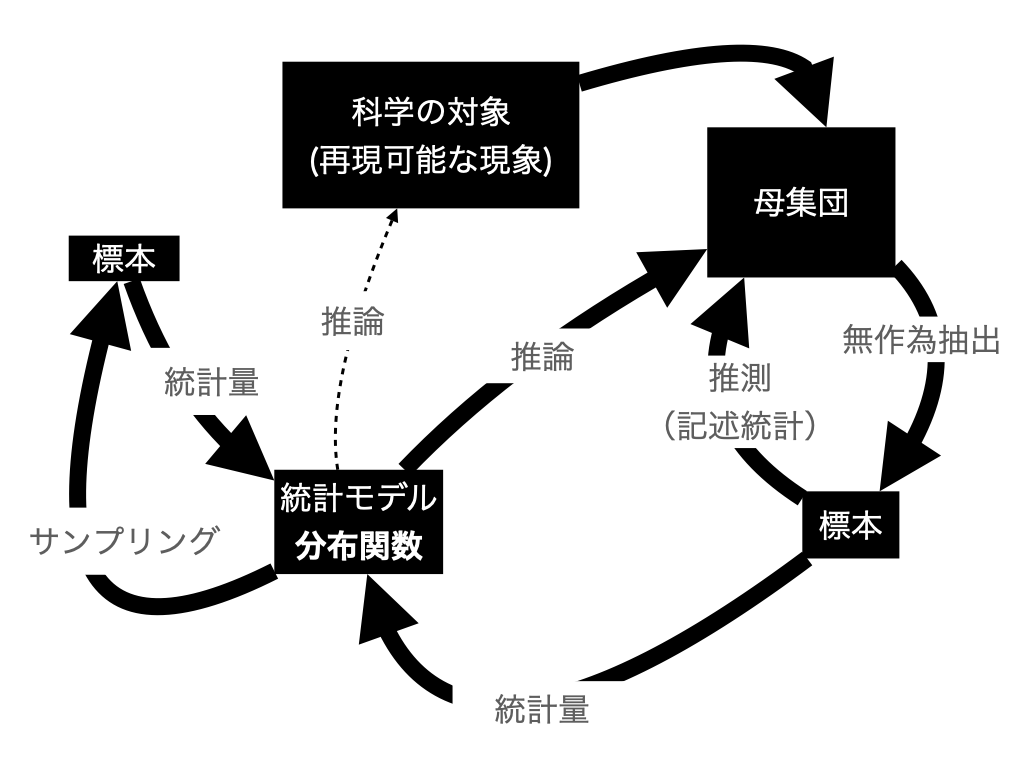
\includegraphics[width=15cm]{./image/01_/conceptual_diagram/conceptual_diagram.002.png}
        \caption{統計モデルによる現象の推測に関する概念図}
        \label{fig:conceptual_diagram_statistics}
    \end{center}
\end{figure}
    

